% Copyright (c) Josua Schmid (2009-2011)
% Dieses Werk ist unter der Creative Commons Attribution-Share Alike 3.0 Unported Lizenz (http://creativecommons.org/licenses/by-sa/3.0/) lizenziert

\documentclass[a4paper]{article}
\usepackage{german}
\usepackage[utf8]{inputenc}
\usepackage{multicol}
\usepackage{graphicx}
\usepackage{amsmath, amsthm, amssymb, amsfonts}
\usepackage{alltt}   % für Pseudocode
\usepackage[all]{xy} % für Graphen

% ZuFa Template laden
\usepackage{tbabstract}


\def\blank{\text{\textvisiblespace}}

%Linie zwischen Multicols
\setlength{\columnseprule}{0.4pt}
\setlength{\columnsep}{0.83cm}

\clubpenalty = 10000
\widowpenalty = 10000
\setlength{\columnseprule}{0pt}

\graphicspath{{./images/}}

\title{Math2I\\Zusammenfassung}
\author{Josua Schmid, Michael Gysel}

\begin{document}
%\maketitle
%\newpage
\tableofcontents
\newpage

\section{Grundlagen}
	\begin{multicols}{2}
	
	\begin{fmerke}[Wichtige Mengenoperationen]
		\renewcommand{\arraystretch}{1.3}
		\begin{tabular}{r|l}
			Durchschnitt & $A \cap B$ \\\hline
			Vereinigung  & $A \cup B$ \\\hline
			Differenz    & $A \setminus B$
		\end{tabular}
	\end{fmerke}
	
	\begin{fmerke}[Verknüpfung]
	\begin{tabular}{ll}
		$\lnot P \vee Q = P \Rightarrow Q$ & wenn $P$ wahr ist, ist $Q$ auch wahr \\
		$P \Rightarrow Q \wedge Q \Rightarrow P$ & $P \Leftrightarrow Q$, $P$ und $Q$ sind äquivalent
	\end{tabular}
	\end{fmerke}
	
	\begin{fmerke}[Morgansche Regel]
	\begin{tabular}{ll}
		$P \wedge Q$ & $= \lnot(\lnot P \vee \lnot Q)$ \\ \hline
		$P \vee Q$ & $=  \lnot(\lnot P \wedge \lnot Q)$ \\ \hline
		$P \rightarrow Q$ & $= \lnot P \vee Q = \lnot\lnot(\lnot P \vee Q)$ \\
		& $= \lnot(P \wedge \lnot Q) = \lnot\lnot Q \vee \lnot P$ \\
		& $= \lnot Q \Rightarrow \lnot P$
	\end{tabular}
	\end{fmerke}
	
	\begin{fmerke}[Prädikate]
	\begin{tabular}{ll}
		$P(x, y) = x < y$ & wahr falls $x$ kleiner als $y$ \\
		$P(n) = n \equiv 0 mod 2$ & wahr falls $n$ gerade
	\end{tabular}
	\end{fmerke}	
	
	\begin{fmerke}[Quantoren]
	\begin{tabular}{ll}
		$\forall (n \in \mathbb{N} \Rightarrow n^2 > 0$ & Das Quadrat jeder natürlichen \\
		$\forall n \in \mathbb{N} (n^2 >0)$ & Zahl $n$ ist grösser 0.\\ \hline
		$\exists w \in \mathbb{R}(x = w^2)$ & Jede positive reelle Zahl $x$ \\
		& hat eine Wurzel w. \\ \hline
		$\forall x > 0 \exists w \in \mathbb{R}(x = w^2)$
	\end{tabular}
	\end{fmerke}

	\begin{fdef}[Wichtige Mengen]
	\begin{tabular}{r|l}
		$\mathbb{N}^+$ & Natürliche Zahlen ohne Null $\{ 1,2,3,\dots \}$ \\\hline
		$\mathbb{N}_0$ & Natürliche Zahlen mit Null $\{ 0,1,2,3,\dots \}$ \\\hline
		$\mathbb{Z}$ & Ganze Zahlen $\{ -2,-1,0,1,2,\dots \}$ \\\hline
		$\mathbb{Q}$ & Rationale Zahlen $\{ \frac{p}{q} \mid p \in \mathbb{Z}, q \in \mathbb{Z} \setminus 0 \}$ \\\hline
		$\mathbb{R}$ & Reelle Zahlen \\\hline
		$\mathbb{C}$ & Komplexe Zahlen
	\end{tabular}
	\end{fdef}
	\end{multicols}

\subsection{Beweise}
	\begin{multicols}{2}

	\begin{falgo}[Beweis durch vollständige Induktion]
	Verankerung: $n=1: \sum\limits_{k=1}^{1}k = 1 = \frac{1(1+1)}{2}$ \\
	(Annahme): $n$ ok? \\
	(Schluss): $n+1$ auch ok? \\
	Induktionsschritt: $n \rightarrow n+1: \sum\limits_{k=1}^{n+1}k = \sum\limits_{k=1}^{n}k + (n+1) = \frac{n(n+1)}{2} + (n+1) = \dots$
	\end{falgo}

	\begin{falgo}[Beweis durch Konstruktion]
	De Seich eifach usrechne.
	\end{falgo}
	
	\begin{falgo}[Beweis durch Widerspruch]
		$A \Rightarrow B$ wird bewiesen durch $\neg B \Rightarrow \neg A$ \\
	\end{falgo}
	
	\textbf{Beispielbeweis:} $\sqrt{z} \in \mathbb{Q}$ mit Annahme: $\sqrt{z} = \frac{p}{q}$
	\begin{align*}
	z = \frac{p^2}{q^2} & \Rightarrow zq^2 = p^2 \\
						& \Rightarrow \text{$p$ gerade} \Rightarrow \text{$p^2$ durch 4 teilbar} \\
						& \Rightarrow \text{$q^2$ gerade} \Rightarrow \text{$q$ gerade} \\
						& \Rightarrow \text{mit 2 kürzen} \\
						& \Rightarrow \textbf{Widerspruch!} \qquad \openbox
	\end{align*}

	\end{multicols}

\subsection{Relationen}
	\begin{multicols}{2}
	
	\begin{fdef}[Relation R von A nach B]
	    $R \subseteq A \times B$ \\
	    Schreibweise: $a \circ b$ für $(a, b) \in R$
	\end{fdef}
	\begin{fdef}[Relation R auf A]
	    $R \subseteq A \times A = A^2$
	\end{fdef}
	
	\begin{feig}[Mögliche Eigenschaften von Relationen]
		\renewcommand{\arraystretch}{1.3}
		\begin{tabular}{r|l}
			symmetrisch     &   $\forall a,b \in A: a \circ b \leftrightarrow b \circ a$\\\hline
			antisymmetrisch &   $\forall a,b \in A: a \circ b \wedge b \circ a \rightarrow a = b$\\\hline
			transitiv       &   $\forall a,b,c \in A: a \circ c \wedge b \circ c \rightarrow a \circ c$ \\\hline
			reflexiv        &   $\forall a \in A: (a,a) \in R$\\\hline
			antireflexiv    &   $\forall a \in A: (a,a) \notin R$
		\end{tabular}
	\end{feig}

	\end{multicols}

\subsection{Äquivalenz- und Ordnungsrelationen}
	\begin{multicols}{2}
	
	\begin{fdef}[Äquivalenzrelation]
	ist eine reflexive, symmetrische und transitive Relation.
	\end{fdef}
	
	\begin{fdef}[Partition]
	    ist eine Mengenfamilie $A_i$ mit $\bigcup A_i = A$
	\end{fdef}

	\begin{fdef}[Partialordnung]
	    Eine reflexive, transitive und anti-symmetrische Relation.
	    Partial, weil nicht alle Element zwingend vergleichbar. Falls doch: \textbf{Totalordnung}
	\end{fdef}
	
	\begin{feig}[Wohlgeordnet]
	    $(A, \le)$ ist wohlgeordnet, wenn jede nichtleere Teilmenge ein kleinstes Element besitzt
	\end{feig}

	\end{multicols}

\subsection{Graphen}
	\begin{multicols}{2}
	
	\begin{fdef}[Grad ($\deg{G}$)]
	Der Grad ist die Anzahl Kanten, welche von einem Knoten ein- und ausgehen.
	\end{fdef}
	
	\begin{fdef}[Beschrifteter, gerichteter Graph]
	besteht aus Ecken $Q \in Q \times Q \times \Sigma$ und Kanten $(q_1,q_2, a)$, falls $\delta(q_1, a) = q_2$
	\end{fdef}

	\end{multicols}

\section{Reguläre Sprachen}

\subsection{Sprachen}
	\begin{multicols}{2}	
	
	\begin{fdef}[Alphabet]
	Ein Alphabet ist eine endliche Menge \\
	Beispiele: \\
	$\Sigma = \{ 0,1 \}$ \\
	$\Sigma = \{ 0 \}$ \\
	$\Gamma = \{ 0,1,w \}$ \\
	$\Delta = \{ a, \dots, z \}$ \\
	\end{fdef}
	\begin{fdef}[Wort]
		Tupel $w$ über dem Alphabet $\Sigma$ \\
		Länge $n$: $n = |w|$
	\end{fdef}
	\begin{fdef}[Leeres Wort $\epsilon$]
		Das leere Wort $\epsilon$ hat die Länge 0.
		Jedes Alphabet enthält das leere Wort: $\Sigma^0 = \{\epsilon \}$
	\end{fdef}
	\begin{fdef}[Menge aller Wörter]
		$\Sigma^* = \{ \sigma \cup \Sigma^1 \cup \Sigma^2 \cup \Sigma^3 \cup \dots \}$
	\end{fdef}
	\begin{fdef}[Sprache $L$]
		$L \subset \Sigma^*$ \\
		Über jedem Alphabet gibt es eine leere Sprache $\emptyset$ und die Sprache $\Sigma^0 = \{\epsilon \}$
	\end{fdef}
	\begin{fdef}[Mengenoperationen]
		Ist $L$ eine reguläre Sprache, dann ist auch $\bar L$ regulär.
		Sind $L_1$ und $L_2$ regulär, dann ist auch $L_1\setminus L_2$
		regulär.
	\end{fdef}
	
	Beispiele... Primzahlen
	
	\begin{fmerke}[C-Standard]
		$\Sigma = $ ASCII \\
		$C = \{w \in \Sigma^* | w \text{ wird vom GCC akzeptiert } \}$
	\end{fmerke}
	\begin{fmerke}[Java]
		$\Sigma = $ Unicode \\
		$J = \{w \in \Sigma^* | w \text{ wird vom javac akzeptiert } \}$
	\end{fmerke}

	\end{multicols}
	

\section{Endliche Automaten und reguläre Sprachen}
	\begin{multicols}{2}

	\begin{fdef}[Deterministischer endlicher Automat (DEA)]
		Ein DEA ist ein Quintupel: 
		$$A = (Q, \Sigma , \delta , q_0, F)$$
		\begin{tabular}{r|l}
		Zustände & Q \\\hline
		Alphabet & $\Sigma$ \\\hline
		Funktion & $\delta: Q \times \Sigma \rightarrow Q: (q,a) \mapsto \delta(q,a)$ \\\hline
		Startzustand & $q_0$ \\\hline
		Akzeptierzustände & $F$ ($\approx$ erfolgreiche Ereignisse)
		\end{tabular}
		(der DEA kann auch als Graph angesehen werden)
	\end{fdef}

	Beispiel Drehkreuz:
	$$A = (Q = \{V,E\}, \Sigma = \{\text{Fahrkarte, Drehen}\}, \delta, V, F = \{V\})$$
	
	\begin{fdef}[Tabellenform]
	Ein Zustandsautomat kann als Tabelle folgendermassen definiert werden. 
	$$Q \times \Sigma = \left[ \begin{array}{cccc}
                          \delta_{1,1} & \dots & \delta_{1,\Sigma} \\
                          \vdots & \ddots & \vdots\\
                          \delta_{Q,1} & \dots & \delta_{Q,\Sigma} \\
                        \end{array} \right]$$
	\end{fdef}
	
	\begin{fsatz}[Reguläre Sprache (Myhill-Nerode)]
	Eine Sprache heisst regulär, wenn es einen DEA gibt, der diese Sprache akzeptiert.
	Dafür muss der DEA folgende Funktion umsetzen: 
	$$\delta: Q\times \Sigma \rightarrow Q:(L(w), a) \mapsto L(wa)$$
	Das heisst, dass $w$ um das Suffix $a$ ergänzt immer noch in der Sprache $L$ ist ($L(wa)$). Die Anzahl der möglichen $a$ muss zudem endlich sein. Das kann in linearer Zeit herausgefunden werden.
	\end{fsatz}

	\begin{fsatz}[Operationen auf Regulären Sprachen] \label{reglangop}
	$L_1, L_2$ regulär $\rightarrow L_1 * L_2$ regulär, wobei $*$ einer logischen Operation oder der Verkettung entspricht.
	\end{fsatz}

	\begin{fmerke}[DEA über einem Alphabet]
	Ein DEA $A$ akzeptiert eine Sprache $L$.
	$$L(A) = \{ w \in \Sigma^* | w \text{ überführt } A \text{ in einen Akzeptierzustand} \}$$
	\end{fmerke}

	\end{multicols}	
	
\subsection{Rekonstruktion eines Automaten}
	\begin{multicols}{2}
	Gegeben: Sprache $L$ über $\Sigma$, $L \subset \Sigma^*$ \\
	Rekonstruktion der Zustandsmenge $Q$ \\
	Annahme: wir haben den Automaten schon gefunden
	
	\begin{falgo}[Beispiel]
		Gegeben ist folgende Sprache $L = \{w \in \Sigma^* \mid |w|_a \equiv 0 \mod 2\}$ und das Alphabet $\Sigma = \{\texttt{a,b}\}$. \\
		Dazu müssen wir die Menge der möglichen $L(w)$ ermitteln: \\
		\begin{tabular}{|c|l|}
			\hline
			$w$ & $L(w)$ \\ \hline
			$\epsilon$ & $L$ \\
			\texttt{a} & $L(\texttt{a}) = \{w \in L^* \mid |w|_a \text{ ungerade}\}$ \\
			\texttt{b} & $L(\texttt{b}) = \{w \in L^* \mid |w|_a \text{ gerade}\}$ \\
			$|w|_a \text{ ungerade}$ & $L(\texttt{a})$ \\
			$|w|_a \text{ gerade}$ & $L)$ \\ \hline
		\end{tabular} \\
		Offenbar gibt es also genau die zwei Zustände $L$ und $L' = L(\texttt{a})$. Ein Zeichen \texttt{a} führt $L$ in $L(\texttt{a})$ über und umgekehrt, das Zeichen \texttt{b} ändert den Zustand nicht: \\
		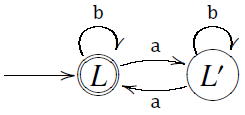
\includegraphics[scale=0.6]{rekonstruktion.png}
	\end{falgo}	
	
	\textbf{Kartesischer Produktautomat}
	\\
	
	Teilautomat $A_1$ für Sprache $L_1 = \{w \in \Sigma^* \mid |w|_0 \text{gerade}\}$ \\
	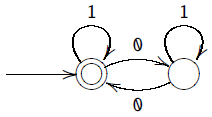
\includegraphics[scale=0.6]{produktautomat_1.png} \\
	Teilautomat $A_2$ für Sprache $L_2 = \{w \in \Sigma^* \mid w \text{ ist eine durch 3 teilbare Binärzahl} \}$ \\
	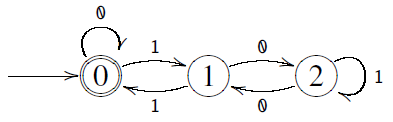
\includegraphics[scale=0.6]{produktautomat_2.png} \\
	Der Produktautomat \\
	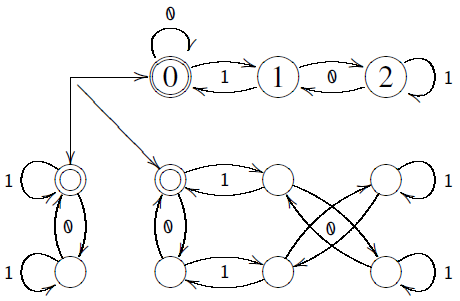
\includegraphics[scale=0.6]{produktautomat_3.png} \\
	Produktautomat umformuliert sodass er auch $L_1 \cup L_2$ akeptiert \\
	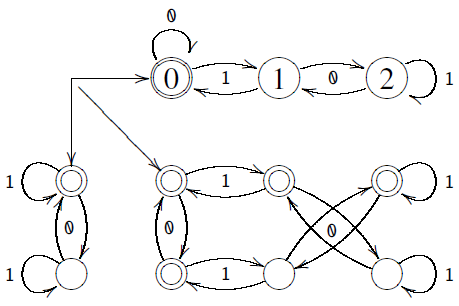
\includegraphics[scale=0.6]{produktautomat_4.png}
		
	\end{multicols}
\newpage
\subsection{Automaten-Minimierung}
	\begin{multicols}{2}
	\label{minimizeautomat}
	\begin{fdef}[Minimaler Automat]
	DEA $A$, $L(A)=L$ mit möglichst wenigen Zuständen.
	\end{fdef}

	\begin{falgo}[Minimierung]
	\textbf{Idee:} Lege überflüssige Zustände zusammen, von denen man auf den gleichen Wegen zu denselben Akzeptierzuständen kommt. \\
	\textbf{Aber:} $L(q_1)=L(q_2)$ herauszufinden ist kompliziert. Es ist einfacher, $L(q_1) \neq L(q_2)$ herauszufinden:
	\begin{enumerate}
		\item Leere Äquivalenzen-Tabelle erstellen
		\item Alle Zustände sind zu sich selbst äquivalent ($\equiv$ markieren)
		\item Akzeptierzustände sind zu keinen anderen Zuständen äquivalent ($\nequiv$ markieren)
		\item Falls von den Zuständen $p$ und $q$ mit dem gleichen Übergang zwei verschiedene, nicht äquivalente Zustände erreicht werden, sind $p$ und $q$ auch als nicht äquivalent zu markieren.
		\item übrigbleibende ,,leere Felder'' $\equiv$ äquivalente Zustände
	\end{enumerate}
	\end{falgo}
	
	\begin{fmerke}[Beispiel]
	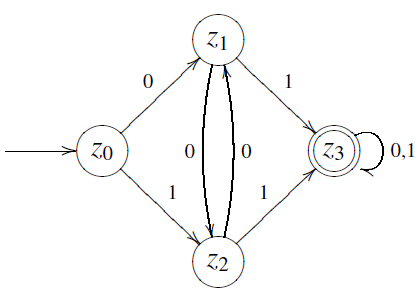
\includegraphics[scale=0.7]{minimal_dea.png}
	\begin{tabular}{lllll}
		& z0 & z1 & z2 & z3 \\
		z0 & $\equiv$ & $\not\equiv$ & $\not\equiv$ & $\not\equiv$ \\
		z1 & $\not\equiv$ & $\equiv$ & X & $\not\equiv$ \\
		z2 & $\not\equiv$ & X & $\equiv$ & $\not\equiv$ \\
		z3 & $\not\equiv$ & $\not\equiv$ & $\not\equiv$ & $\equiv$
	\end{tabular} \\
	Jeder Zustand ist mit sich selbst äquivalent. \\
	Endzustände sind nicht mit Zuständen äquivalent, welche keine Endzustände sind. \\
	In diesem Beispiel bleiben nur noch 2 Kombinationen (X) offen. Von beiden Paaren wird immer auf den jeweils anderen oder z3 überführt. Daher sind die Zustände äquivalent. \\
	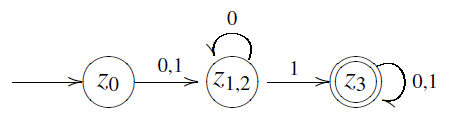
\includegraphics[scale=0.6]{minimal_dea_2.png}
	\end{fmerke}
	\end{multicols}
	
\subsection{Regularität}
	\begin{multicols}{2}
	Eine Sprache ist regulär, wenn man
	\begin{itemize}
		\item einen Automaten bauen kann
		\item einen regulären Ausdruck angeben kann
	\end{itemize}
	der die Sprache akzeptiert.
	
	\begin{fdef}[Pumping Lemma (PL)]
	Das PL beweist, ob eine Sprache nicht regulär ist.
	\end{fdef}
	
	\begin{fmerke}[Prinzip der Beweisführung]
	Ein ,,langes'' Wort $w$, für das gilt $|w| \le |Q|$, bildet eine Schleife im Automaten.
	
	$$\text{Zerteile $w$ in $xyz$}$$
	$$|xy| \ge |Q|$$
	$$|y| \ge 1$$
	
	Neue Wörter basteln, indem wir die Schleife ($y$) weglassen: 
	$$xz \in L$$
	oder mehrmals durch die Schleife laufen:
	$$xyyz \in L \Rightarrow xy^kz \in L \qquad \forall k \in \mathbb{N}$$				
	\end{fmerke}

	
	\begin{falgo}[Pumping Lemma Ablauf]
	$L$ regulär $\Rightarrow \exists N$ pumping length falls $w \le N \Rightarrow w=xyz$ mit 
	\begin{enumerate}
		\item $|xy| \le N$
		\item $|y| \ge 1$
		\item $xy^{k}z \in L \forall k \ge 0$
	\end{enumerate} 
	\end{falgo}
	
	\textbf{Beweisbeispiel:}
	\begin{itemize}
		\item Anwendung: $L=\{0^n1^n | n \in \mathbb{N}\}$ nicht regulär 
		\item Widerspruchsbeweis: Annahme $L$ regulär
		\item PL: $N$
		\item Behauptung: $w=0^n1^N$   $|w| = 2N \le N$   $|0^N| = |1^N|$
		\item PL: $|0^N| \neq |1^N|$
	\end{itemize}
	
	\end{multicols}	
	
\subsection{Nicht deterministische Automaten}
	\begin{multicols}{2}
	
	\begin{fdef}[Nichtdeterministischer endlicher Automat (NEA)]
		ein Nichtdeterministischer endlicher Automat ist 
		$$A = (Q, \Sigma, \delta, q_0, F)$$
		mit
		$$\delta : Q \times (\Sigma \cup \{\epsilon\}) \rightarrow P(Q)$$
		Jeder DEA ist ein NEA. Bei einem DEA:
		\begin{align*}
			\delta(q,\epsilon) = \emptyset \qquad & \forall q \in Q \\
			|\delta(q,a)| = 1              \qquad & \forall q \in Q, a \in \Sigma
		\end{align*}
	\end{fdef}
	
	Beispiel für eine nicht Reguläre Sprache: Ganzzahlautomat
	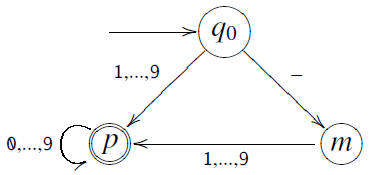
\includegraphics[scale=0.7]{nea_beispiel.png}
	Ein NEA ohne den Zustand $e$.
	\end{multicols}
	
\subsection{Transformation NEA $\rightarrow$ DEA}
	\begin{multicols}{2}
	
	\textbf{Idee:}
	\begin{enumerate}
		\item Suche einen Algorithmus, der einen NEA ohne $\epsilon$-Übergänge in einen DEA umwandelt.
		\item Modifiziere den Algorithmus so, dass er auch mit dem NEA inkl. $\epsilon$-Übergängen umgehen kann.
	\end{enumerate}

	Der konstruierte DEA muss darüber Buch führen, in welchen Zuständen der NEA sein könnte.
	$\Rightarrow$ Zustände des DEA sind also Teilmengen von $Q$.
	
	\begin{fsatz}
		\begin{align*}
		A = (Q, \Sigma, \delta, q_0, F)      \qquad & \text{ein NEA ohne $\epsilon$-Übergänge.} \\
		A' = (Q', \Sigma, \delta', q'_0, F') \qquad & \text{ein DEA}
		\end{align*}
		$$L(A) = L(A')$$
		$$\delta': Q' \times \Sigma \rightarrow Q' : (M,a) \rightarrow \bigcup_{q \in M}^{}{\delta(q,a)} = \delta(M,a)$$
		$$F' = \{M \in Q' \mid M \cap F \neq \emptyset \}$$
	\end{fsatz}
	
	\begin{falgo}[Überprüfung der Äquivalenz zweier Automaten]
	\begin{enumerate}
		\item ev. NEA in DEA umwandeln
		\item Minimaler Automat erstellen (siehe \ref{minimizeautomat})
		\item Mit Graphentabelle auf Gleichheit überprüfen
	\end{enumerate}
	\end{falgo}
	
	\end{multicols}	
	
\subsection{Reguläre Ausdrücke}
	Es sei $r$ ein Regulärer Ausdruck, und $L(r)$ die Sprache, die dazu passt. Alle Wörter aus $L(r)$ haben die Länge 1, damit ist $L(r)$ regulär.
	
	\begin{multicols}{2}
	\begin{tabular}{|l|l|}
		\multicolumn{2}{c}{\textbf{Zeichen}} \\
		\hline
		Ausdruck $r$     & Bedeutung \\\hline
		\texttt{a}       & Zeichen \texttt{a} $\in \Sigma$ \\
		\texttt{.}       & beliebiges Zeichen aus $\Sigma$ \\
		\texttt{[aeiou]} & Zeichen aus $\{ \texttt{a},\texttt{e},\texttt{i},\texttt{o},\texttt{u} \} \subset \Sigma$ \\
		\texttt{[1-9]}   & positive Ziffern \\
		$\epsilon$       & leeres Wort \\
		$\emptyset$      & leere Sprache \\\hline
	\end{tabular}
	
	\begin{tabular}{|l|c|l|}
		\multicolumn{3}{c}{\textbf{Operationen}} \\\hline
		                & Ausdruck  & reguläre Operation \\\hline
		Verkettung      & $r_1r_2$  & $L(r_1)L(r_2)$ \\
		Alternative     & $r_1|r_2$ & $L(r_1) \cup L(r_2)$ \\
		Stern-Operation & $r_1^*$   & $L(r_1)^* =$ beliebige Anzahl \\\hline
	\end{tabular}
	\end{multicols}

\newpage	
\subsection{Verallgemeinerter NEA (VNEA)}
	\begin{multicols}{2}
	Ein VNEA ist ein NEA, der reguläre Ausdrücke akzeptiert. Der VNEA besteht aus den zwei Zuständen $q_{\text{start}}$ und $q_{\text{accept}}$, welche mit dem $r$-Pfeil verbunden sind.	
	\begin{falgo}[Umwandlung: NEA $\rightarrow$ VNEA]
		\begin{enumerate}
			\item Füge zum NEA einen neuen Startzustand hinzu mit $\epsilon$-Pfeil zum alten Startzustand.
			\item Füge zum NEA einen neuen Akzeptierzustand hinzu mit $\epsilon$-Pfeil zum alten Akzeptierzustand.
			\item Reduziere den NEA indem die alten Zustände der Reihe nach ,,herausgerissen'' und ein Alternativweg mit entsprechendem RegExp-Operator angeschrieben wird.
		\end{enumerate}
	\end{falgo}
	
	Für das Beispiel wird ein DEA anstelle eines NEA verwendet. Das Prinzip bleibt aber dasselbe. \\		
	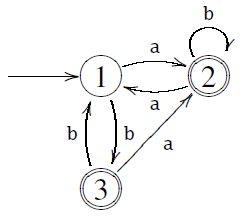
\includegraphics[scale=0.6]{vnea_beispiel_1.png} \\
	\\
	Im ersten Schritt fügen wir die neuen Start- und Akzeptierzustände hinzu, die Zustände 2 und 3 sind damit nicht mehr Akzeptierzustände. \\
	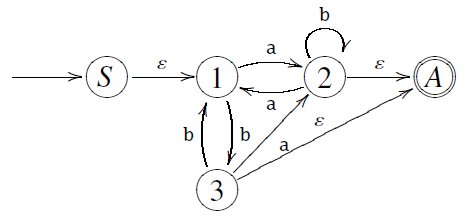
\includegraphics[scale=0.5]{vnea_beispiel_2.png} \\
	\\
	Jetzt entfernen wir nacheinander alle ''inneren'' Zustände. Wir beginnen mit dem Zustand 1, dabei sind die Pfade S -1-2, S -1-3, 2-1-3, 3-1-2, 2-1-2 und 3-1-2 zu
berücksichtigen. \\
	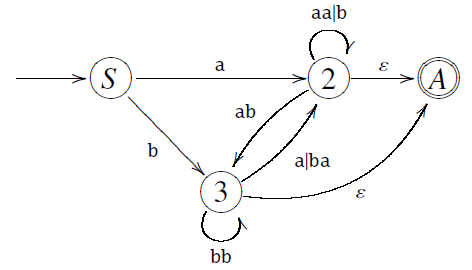
\includegraphics[scale=0.5]{vnea_beispiel_3.png} \\
	\\
	Jetzt wird der Zustand 2 entfernt, dabei sind die Pfade S -2-A, S -2-3, 3-2-A, und 3-2-3 zu berücksichtigen. \\
	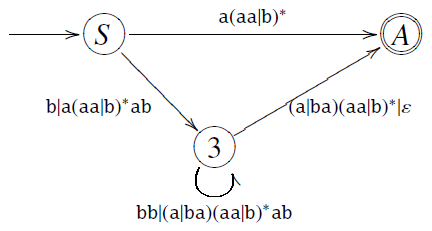
\includegraphics[scale=0.5]{vnea_beispiel_4.png} \\
	\\
	Jetzt muss nur noch der Zustand 3 entfernt werden. \\
	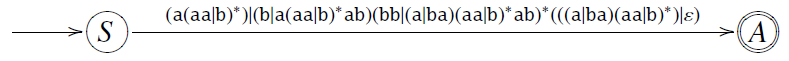
\includegraphics[scale=0.35]{vnea_beispiel_5.png}
		
	\end{multicols}



\section{Stackautomaten und Kontextfreie Sprachen}


\subsection{Regeln (Grammatik)}
	\begin{multicols}{2}
	
	\begin{fdef}[Kontextfreie Grammatik]
	Eine Kontextfreie Grammatik ist ein Quadrupel $(V, \Sigma, R, S)$ mit
	\begin{itemize}
		\item $V$ ist eine endliche Menge von Variablen
		\item $\Sigma$ ist eine endliche Menge von Zeichen (Terminalsymbole)
		\item $R$ ist eine Menge von Regeln
		\item $S \in V$ ist die Startvariable
	\end{itemize}
	\end{fdef}
	
	\textbf{Beispiel einer Regel:}
	$$A \rightarrow BCx \text{ (wobei $B,C \in V$ und $x \in \Sigma$)}$$
	
	\textbf{Beispiel einer Kontextfreien Grammatik:} \\
	Korrekte Klammerung mit $a=$\texttt{(} und  $b=$\texttt{)}
	\begin{align*}
		A & \rightarrow \epsilon \\
		A & \rightarrow AA \\
		A & \rightarrow aAb
	\end{align*}
	Dazu äquivalent wäre: $A \rightarrow \epsilon \mid AA \mid (A)$

	\begin{fdef}[Kontextfreie Sprache]
	Die Menge aller Wörter die von einer Kontextfreien Grammatik durch Ableitung erzeugt werden können. Ableitung ist das ersetzen aller Variablen durch Terminalsymbole.
	$$L(G)  = \{ w \in \Sigma^* \mid S \stackrel{*}{\Rightarrow} u \}$$
	\end{fdef}

	\begin{fmerke}[Beispiel: Natürliche Zahlen]
	$\mathbb{N}$ enthält Worte aus 
	$\{\texttt{0},\texttt{1},\texttt{2},\texttt{3},
	   \texttt{4},\texttt{5},\texttt{6},
	   \texttt{7},\texttt{8},\texttt{9} \}$
	, welche aus folgenden Grammatikregeln erzeugt werden:
	\begin{align*}
		A & \rightarrow Z \\
		  & \rightarrow NZ \\
		Z & \rightarrow \texttt{0} \mid \texttt{\dots} \mid \texttt{9}
	\end{align*}
	\end{fmerke}
	
	\begin{fmerke}[Kontextfreiheit]
	\begin{itemize}
		\item Die Regeln einer Kontextfreien Grammatik werden ohne externe Abhängigkeiten angewendet. Eine Regel wie $aA \rightarrow AA$ wäre nicht kontextfrei und daher nicht erlaubt. \\
		\item Für Kontextfreie Sprachen gelten die gleichen Operationen wie für Reguläre Sprachen (siehe \ref{reglangop})
		\item Alle regulären Sprachen haben eine Kontextfreie Grammatik.
	\end{itemize}
	\end{fmerke}
	
	\end{multicols}
	
\subsection{Chomsky Normalform}
	\begin{multicols}{2}
	
	\begin{fdef}[Definition]
	Eine Kontextfreie Grammatik ist in Chomsky Normalform, wenn sie Regeln von folgender Form besitzt:
	\begin{align*}
		S & \rightarrow \epsilon \\
		A & \rightarrow BC \\
		A & \rightarrow a
	\end{align*}
	\end{fdef}	
	
	\begin{falgo}[Umwandlung: Kontextfreie Grammatik $\rightarrow$ Chomsky Normalform]
		\begin{enumerate}
			\item Ersetze $S \rightarrow \epsilon$ durch $S_0 \rightarrow \epsilon$ und $S_0 \rightarrow S$, wobei \\
			$S =$ alte Startvariable und $S_0 =$ neue Startvariable
			\item Lösche alle Regeln der Form $A \rightarrow \epsilon$ (nur $S_0 \rightarrow \epsilon$ bleibt bestehen). Für jede Regel, die ein solches $A$ auf der rechten Seite enthält, wird eine Regel hinzugefügt, in der das $A$ gestrichen wurde.\\
			      z.B.: $A \rightarrow \epsilon, B \rightarrow AC$ wird zu $B \rightarrow C, B \rightarrow AC$
			\item Ersetze Regeln mit nur einer Variable auf der rechten Seite \\
			      z.B.: $A \rightarrow B, B \rightarrow CD$ wird zu $A \rightarrow CD, B \rightarrow CD$
			\item Ersetze Verkettungen durch neue Variablen \\
			      z.B.: $S \rightarrow ASA$ wird zu $S \rightarrow AT, T \rightarrow SA$
			\item Ersetze Terminalsymbole durch Regeln \\
				  z.B.: $Z \rightarrow \texttt{0}Z_1$ wird zu $Z_0 \rightarrow \texttt{0}$, $Z \rightarrow Z_0Z_1$
		\end{enumerate}
	\end{falgo}
	
	\end{multicols}	
	
\subsection{Parsing}
	\begin{fmerke}[Parse Tree]
	Der Ableitungsbaum eines Wortes einer kontcfg to stackextfreien Sprache ist eine Darstellung der verwendeten Produktionsregeln in Baum-Struktur. Dabei wird ein String ,,geparst''.
	
	ev. Bsp zu Ableitungsbaum

	\begin{itemize}
		\item Äquivalente Ableitungen haben den selben Ableitungsbaum.
		\item Hat eine Sprache Wörter mit verschiedenen Ableitungen, heisst sie mehrdeutig.
	\end{itemize}
	\end{fmerke}
	
	\begin{falgo}[Ein deterministischer Parse Algorithmus (CYK)]
	\begin{multicols}{2}
	Der CYK-Algorithmus entscheidet, ob ein Wort $w$ in einer Kontextfreien Sprache ist. Die Laufzeit beträgt $\mathcal{O}(n^3)$. \\
	\textbf{Idee}: Das Wort $w=w_1w_2$ wird unterteilt in $w_1$ und $w_2$. Dann wird geprüft, ob die Regeln der Grammatik auf $w_1$ und $w_2$ zutreffen. Das geschieht rekursiv.
	
	Input: $A \in V, w \in \Sigma^*$ \\
	Output: kann $w$ aus $A$ abgeleitet werden? $A \stackrel{*}{\Rightarrow} w$ ?
	Spezialfall: $S, w \Rightarrow w \in L(G)$ ?
	Annahme: Grammatik in CNF
	nur Regeln $A \rightarrow BC$
	$A \rightarrow a$
	
	\columnbreak
	
	\begin{alltt}
boolean cyk(Variable \(A\), Wort \(w\)) \{
  falls \(|w|>1\): für jede Aufteilung \(w=w_1 w_2\) 
              und jede Regel \(A \rightarrow BC\) \{
    teste: \(B \stackrel{*}{\Rightarrow} w_1\)
           \(C \stackrel{*}{\Rightarrow} w_2\)
    falls ja, return true, sonst false
  \}
\}\end{alltt}
	\end{multicols}
	\end{falgo}

\subsection{Stackautomaten}
	\begin{multicols}{2}
	
	Die Kontextfreie Sprache $L = \{0^n1^n | n \in \mathbb{N}\}$ ist mit einem Stack erkennbar. 
	Ein Stackautomat ist immer nichtdeterministisch.
	\begin{fdef}[Stackautomat]
		$P = (Q, \Sigma, \Gamma, \delta, q_0, F)$  \\
		$\Gamma$ das Stackalphabet \\
		$$\delta: Q \times \Sigma_\epsilon \times \Gamma_\epsilon \longrightarrow P(Q \times \Gamma_\epsilon)$$

		Wenn $\Sigma$ oder $\Gamma$ $\epsilon$ nicht enthalten:
		$$\Sigma_{\epsilon} = \Sigma \cup \epsilon$$
		$$\Gamma_{\epsilon} = \Gamma \cup \epsilon$$
	\end{fdef}
	
	\begin{fmerke}[Operationen auf dem Stackgraphen]
	Input $a$ definiert den Übergang.
	\begin{itemize}
		\item c wird auf den Stack gelegt
		      \[ \entrymodifiers={++[o][F]}
		         \xymatrix{   p \ar[r]^{a,\epsilon \rightarrow c} & q   } \]

		\item b wird vom Stack entfernt
		      \[ \entrymodifiers={++[o][F]}
		         \xymatrix{   p \ar[r]^{a,b \rightarrow \epsilon} & q   } \]

		\item Stack bleibt unverändert
		      \[ \entrymodifiers={++[o][F]}
		         \xymatrix{   p \ar[r]^{a,\epsilon \rightarrow \epsilon} & q   } \]
	\end{itemize}
	\end{fmerke}
	
	\begin{fmerke}[Beispiel $L=\{0^n1^n | n \in \mathbb{N}\}$]
	Um Einen und Nullen geht folgendermassen: Lege alle Nullen auf den Stack. Dann entferne pro eingehender Eins eine Null vom Stack. Wenn der Stack am Schluss leer ist, genügte der Input der Grammatik.\\
	$$\Gamma = \{ \texttt{0}, \texttt{1}, \texttt{\$} \}$$
	\texttt{\$} markiert den Anfang des Stack
	\[ \entrymodifiers={++[o][F]}
	   \xymatrix{   \ar[r]^{\epsilon,\epsilon \rightarrow \texttt{\$}} & \ar@(ur,dr)^{\texttt{0}, \epsilon \rightarrow \texttt{0}} \ar[d]^{\epsilon, \epsilon \rightarrow \epsilon} \\
	   	            & \ar[l]^{\epsilon, \texttt{\$} \rightarrow \epsilon} \ar@(ur,dr)^{\texttt{1}, \texttt{0} \rightarrow \epsilon}
	} \]
	\end{fmerke}
	\end{multicols}

	\begin{falgo}[Umwandlung: Grammatik $\rightarrow$ Stackautomat]
	\begin{multicols}{3}

	Auch genannt Blüemlialgorithmus. Setze alle Regeln einzeln in einen Automaten um. \\\hspace{3mm}
	
	\textbf{Beispiel:}
	
	\begin{align*}
	E & \rightarrow E\texttt{+}T \\
	E & \rightarrow T \\
	T & \rightarrow TxF
	\end{align*}

	\columnbreak

	Für jede Regel:
	\begin{displaymath}
	\entrymodifiers={++[o][F]}
    \xymatrix{
        *+{}   & *+{}   & \ar[r]^{\epsilon,\epsilon \rightarrow x} & \ar[ld]^{\epsilon,\epsilon \rightarrow T} \\
        \ar[r]^{\epsilon, \epsilon \rightarrow \texttt{\$}} & \ar[r]^{\epsilon,\epsilon \rightarrow E } & B \ar@(ul,u)^{\epsilon, E\rightarrow T} \ar[r]^{\epsilon,\texttt{\$} \rightarrow \epsilon } \ar[u]^{\epsilon,T\rightarrow F\quad } \ar[d]^{\epsilon,\epsilon \rightarrow T } & \\
		*+{}   & *+{}   & \ar[r]^{\epsilon,\epsilon \rightarrow \texttt{$+$} } & \ar[lu]^{\epsilon,\epsilon \rightarrow E }      
    }
	\end{displaymath}
	
	\columnbreak

	und zusätzlich für jedes Terminalsymbol $\xi$:
	\begin{displaymath}
	\entrymodifiers={++[o][F]}
    \xymatrix{
    	B \ar@(lu,u)^{\xi_1,\xi_1 \rightarrow \epsilon}
    	  \ar@(ru,r)^{\xi_2,\xi_2 \rightarrow \epsilon}
    	  \ar@(rd,d)^{\xi_3,\xi_3 \rightarrow \epsilon}
    	  \ar@(ld,l)^{\xi_4,\xi_4 \rightarrow \epsilon}
    }
	\end{displaymath}
	\end{multicols}	
	\end{falgo}
	
	\begin{falgo}[Umwandlung: Stackautomat $\rightarrow$ Grammatik]
	\textbf{ev. hinzuzufügen}
	\end{falgo}
	
	\begin{fdef}[Pumping Lemma für Kontextfreie Sprachen]
	Es gibt eine Pumping Length $N$, so dass jedes Wort $w \in L$ mit $|w| \geq N$ zerlegt werden kann in fünf Teile $w = uvxyz$
	\begin{itemize}
		\item $|vy| \ge 0$
		\item $|vxy| \leq N$
		\item $uv^kxy^kz \in L$ für alle $k \in \mathbb{N}$
	\end{itemize}
	\end{fdef}

	
	
\subsection{Real World Parser}
	\begin{multicols}{2}

	\begin{falgo}[Shift Reduce]
	Der Shift Reduce Parser vergleicht schrittweise die auf dem Stack befindlichen Zeichen mit den Regeln der Grammatik. Sobald er eine Übereinstimmung zwischen Folge und Regel gefunden hat, wendet er die Regel an, reduziert das Wort zu einer Variable und legt das Resultat auf den Stack.
	\end{falgo}

	\textbf{Beispiel:} \\\vspace{2mm}
	Sprache: $L=\{0^n1^n \mid n \geq 0 \}$ \\
	Grammatik: \begin{align*} 
		w & \rightarrow 0w1 \\
  & \rightarrow 01
	\end{align*}

	\begin{tabular}{|l|l|l|} \hline
		Input  & Stack & Operation \\\hline
		000111 &       & Schiebe \\
		00111  & 0     & Schiebe \\
		0111   & 00    & Schiebe \\
		111    & 000   & Schiebe \\
		11     & 0001  & Reduziere mit Regel 2 \\
		11     & 00w   & Schiebe \\
		1      & 00w1  & Reduziere mit Regel 1 \\
		1      & 0w    & Schiebe \\
      & 0w1   & Reduziere mit Regel 1 \\
      & w     & Schiebe \\\hline
	\end{tabular}

	\begin{falgo}[LR(0)]
	Matching auf Regelebene, mit Codierung der relevanten Stackinhalte als Zustände im Automaten. \\
	\textbf{Kapier ich noch nicht!} \\
		Beispiel: $L = \{0^n 1^n \}$
		$$ W \rightarrow \epsilon $$
		$$ W \rightarrow 0W1 $$
	\end{falgo}

	\begin{fmerke}[Parsertabelle]
	Eine Parsertabelle listet die LR(0)-Elemente und die Konsequenzen wenn eines davon auftritt (Schieben oder Regel anwenden). Eigentlich ist sie nichts anderes als ein Handbuch für den Stackautomaten.
	\end{fmerke}

	\begin{fmerke}[Konflikte]
	\begin{itemize}
		\item Reduce-Reduce-Konflikt: $A \rightarrow 01, B \rightarrow 01$
		\item Shift-Reduce-Konflikt: $A \rightarrow 1, A \rightarrow 1A$ \\
     ($A \rightarrow 1, A \rightarrow A1$ ergäbe keine Probleme)
	\end{itemize}
	\end{fmerke}

	$L = \{a^n b^n c^n | n \in \mathbb{N}\}$ ist nicht kontextfrei

	\end{multicols}	
	

\newpage
\section{Turing-Maschinen}
	\begin{multicols}{2}
	
	\begin{fdef}[Turing-Maschine]
		Die Turingmaschine ist ein endlicher Automat, der anstatt eines Stack ein unendlich grosses Band als Speicher besitzt. Sie wird definiert durch das 7-Tupel
		$M=(Q,\Sigma,\Gamma,\delta,q_0,q_{\text{accept}},q_{\text{reject}})$.
		wobei gilt:
		
		\vspace{2mm}
		\begin{tabular}{r|l}
		$Q$      & Menge der Zustände \\\hline
		$\Sigma$ & Inputalphabet (ohne ,,blank''-Zeichen) \\\hline
		$\Gamma$ & Bandalphabet, es gilt $\blank \in \Gamma$ und $\Sigma \subset \Gamma$ \\\hline
		$\delta$ & Übergangsfunktion $\delta: Q \times \Gamma \rightarrow Q \times \Gamma \times \{ L,R \}$ \\\hline
		$q_0$               & Startzustand \\\hline
		$q_{\text{accept}}$ & Akzeptierzustand \\\hline
		$q_{\text{reject}}$ & Ablehnungszustand
		\end{tabular}
		\vspace{2mm}
		
		Die Übergangsfunktion liefert jeweils ein Tripel (neuer Zustand, neuer Bandinhalt, Links- oder Rechtsbewegung L/R). Jede TM mit Bandalphabet $\Gamma$ kann auf einer TM mit $\Gamma = \{\texttt{0},\texttt{1},\blank\}$ simuliert werden.
	\end{fdef}
	
	\begin{fdef}[Nichtdeterministische Turingmaschine]
		Die nichtdeterministische TM besitzt folgende Übergangsfunktion: $\delta: Q \times \Gamma \rightarrow \mathcal{P}(Q \times \Gamma \times \{ L,R \})$. Der Automat muss also bei jedem Übergang aus allen möglichen wählen.
		Jede nichtdeterministische Turingmaschine ist äquivalent zu einer deterministischen
		Turingmaschine.
	\end{fdef}
	
	\begin{fdef}[Entscheider]
	Ein Entscheider ist eine Turingmaschine, die auf jedem Input $w \in \Sigma^*$ anhält. Eine Sprache heisst entscheidbar, wenn ein Entscheider sie erkennt.
	\end{fdef}
	
	\begin{fmerke}[Zustandsautomat]
	Für die Übergangsfunktion $\delta(q_1,1) = (q_2,b,R|L)$ schreiben wir:
		\[ \entrymodifiers={++[o][F]}
			         \xymatrix{   q_1 \ar[r]^{a \rightarrow b,R|L} & q_2   } \]
	$a = $ Zeichen gelesen vom Band \\
	$b = $ Zeichen zu Schreiben auf Band
	\end{fmerke}
	
	\end{multicols}	
	
\subsection{Aufzähler}
	\begin{multicols}{2}
	\begin{fdef}[Aufzähler]
	Eine TM mit einem Drucker heisst Aufzähler \\
	$\Rightarrow$ Ausgaben von beliebig vielen Wörtern auf den Drucker \\
	\hspace{2mm}
	Eine Turing-erkennbare Sprache wird von einem Aufzähler aufgezählt und umgekehrt.
	\end{fdef}
	
	\begin{falgo}[Umwandlung: Aufzähler $\rightarrow$ TM]
	Ein Aufzähler entspricht einer TM mit 2 Bändern:
	\begin{itemize}
		\item Band 1: $w$
		\item Band 2: Arbeitsband des Aufzählers
	\end{itemize}
		
	\textbf{Algorithmus:}
	\begin{enumerate}
		\item Aufzähler laufenlassen
		\item Bei jedem Druckbefehl: Vergleiche Output mit $w$ falls gleich: $q_{accept}$
	\end{enumerate}
	Falls das Wort zur Sprache gehört, wird der Aufzähler es früher oder später aufzählen.
	\end{falgo}
	\end{multicols}	

\subsection{Berechenbarkeit / Abzählbarkeit}
	Eine Zahl ist berechenbar, wenn ein Aufzähler existiert, der ,,mit der Zeit'' alle Stellen der Zahl ausdruckt.
	
	\begin{multicols}{2}
	\begin{fsatz}[Berechenbare Zahlen]
	\begin{itemize}
		\item rationale Zahlen
		\item Quadratwurzeln
		\item Algebraische Zahlen \small{(Lösungen von Polynomen mit rationalen Koeffizienten)}
	\end{itemize}
	\end{fsatz}
	\begin{fsatz}[Nicht berechenbare Zahlen]
	Die Menge der nicht berechenbaren Zahlen ist überabzählbar.\\
	Beweis: $\mathbb{R}$ überabzählbar und $\{$TM$\}$ abzählbar
	\end{fsatz}

	\begin{fmerke}[Abzählbarkeit]
	Sachverhalte, die mit dem Prinzip der Abzählbarkeit erklärt werden:
	$$\infty \neq \infty$$
	$$|\{1,2,3\}| = 3$$
	$$|\mathbb{N}| \stackrel{?}{=} |\mathbb{R}|$$
	\end{fmerke}
	\end{multicols}
	
	\begin{fmerke}[Hilbert Hotel]
		\begin{itemize}
			\item $n$ Gäste: Alle um $n$ verschieben
			\item $\mathbb{N}$ Gäste: Alle Gäste von den Zimmern $n$ nach $2n$ verschieben
			\item $\mathbb{N} \times \mathbb{N}$ Gäste: Kolonnen diagonal aufrufen und einsortieren
			\item $\mathbb{R}$ Gäste: Können nicht mehr untergebracht werden
		\end{itemize}
		Konsequenz: Eine unendliche Menge ist offenbar so gross, dass man darin immer noch Platz genug für eine Kopie der ganze Menge finden kann. Oder anders herum: endliche Mengen sind solche, in denen man niemals Platz finden könnte.
		%Video: \\
		%http://www.veoh.com/watch/v68132393EgApqc2
	\end{fmerke}
	
	\begin{fdef}[Abzählbarkeit  Überabzählbarkeit]
	\begin{enumerate}
		\item Eine unendliche Menge $A$ heisst abzählbar unendlich, wenn sie gleichmächtig ist wie $\mathbb{N}$
		\item $A$ heisst überabzählbar unendlich, wenn es keine Bijektion zwischen $\mathbb{N}$ und $A$ gibt.
		\item Die Vereinigung von endlich vielen abzählbaren Mengen ist abzählbar.
		\item Das kartesische Produkt zweier abzählbaren Mengen ist abzählbar.
		\item $\mathbb{Z}$ und $\mathbb{Q}$ sind abzählbar unendlich.
		\item $\mathbb{R}$ ist überabzählbar unendlich.
		\item $A$ eine abzählbar unendliche Menge, dann ist $\mathcal{P}(A)$ überabzählbar.
		\item $\Sigma^*$ ist abzählbar unendlich
		\item Die Menge der Sprachen über dem Alphabet $\Sigma$ ist überabzählbar unendlich.
	\end{enumerate}
	\end{fdef}
	
	\begin{fmerke}[Anwendung]
	Sei $\Sigma$ ein festes Alphabet, so sind folgende Mengen abzählbar unendlich:
	\begin{enumerate}
		\item alle DEA, NEA, Stackautomaten und TM
		\item alle regulären und alle kontextfreien Sprachen
		\item alle kontextfreien Grammatiken
	\end{enumerate}
	\end{fmerke}

	Es gibt nur abzählbar viele Turing Maschinen $\Rightarrow$ die meisten Sprachen können nicht mit einer Turing Maschine erkannt werden.

	
\section{Entscheidbarkeit}

	\begin{multicols}{2}
	
	\begin{fmerke}[Übersicht über Sprachen]
	regulär $\subset$ kontextfrei $\subset$ entscheidbar (rekursiv) $\subset$ TM erkennbar (rekursiv aufzählbar) $\subset$ überabzählbar
	\end{fmerke}
	
	Ein Problem muss zuerst immer umformuliert werden zu einem Sprachproblem $A$.
	z.B.: ,,Wird ein Wort $w$ von DEA $A$ akzeptiert?''
	
	\end{multicols}

\subsection{Entscheidbare Probleme für reguläre Sprachen}
	\begin{multicols}{2}
	\begin{falgo}[Akzeptanzproblem]
		$A_{\text{DEA}} = \{ \langle B,w \rangle \mid \text{$B$ ist ein DEA, $B$ akzeptiert $w$} \}$ \\
		$A_{\text{NEA}} = \{ \langle B,w \rangle \mid \text{$B$ ist ein NEA, $B$ akzeptiert $w$} \}$ \\
		$A_{\text{REX}} = \{ \langle R,w \rangle \mid \text{$R$ ist  ein Regulärer Ausdruck und akzeptiert $w$} \}$
		\begin{enumerate}
			\item Wandle $B$ in einen DEA um falls nötig
			\item Simuliere $B$ auf einer TM mit Input $w$ \\
			$\rightarrow$ falls $B$ akzeptiert: $q_{accept}$ \\
			$\rightarrow$ sonst: $q_{reject}$
		\end{enumerate}
	\end{falgo}
	
	\begin{falgo}[Leerheitsproblem]
		 $E_{\text{DEA}} = \{ \langle A \rangle \mid \text{$A$ ist ein DEA und $L(A)=\emptyset$} \}$
		 \begin{enumerate}
			\item Zeichne den Automaten
			\item markiere Startzustand
			\item markiere alle in einem Schritt erreichbaren Knoten
			\item Wiederhole 3. bis keine neuen Zustände mehr markiert werden können.\\
			$\rightarrow$ falls ein Akzeptierzustand erreicht wurde: $q_{reject}$ \\
			$\rightarrow$ sonst $q_{accept}$
		\end{enumerate}
	\end{falgo}
	
	\begin{falgo}[Gleichheitsproblem]
		$EQ_{\text{DEA}} = \{ \langle A,B \rangle \mid \text{$A$ und $B$ sind DEAs und $L(A)=L(B)$} \}$
		\begin{enumerate}
			\item Erzeuge minimale Automaten ($A' \leftarrow A, B' \leftarrow B$)
			\item Falls $A' = B' \Rightarrow q_{accept}$, sonst $q_{reject} $
		\end{enumerate}
		Beweis 2: über Mengendefinition. Für Mengendefinitionen gibt es einen Entscheider.
	\end{falgo}
	\end{multicols}

\subsection{Entscheidbare Probleme für kontextfreie Sprachen}
	\begin{multicols}{2}
	\begin{falgo}[Akzeptanzproblem]
		$A_{\text{CFG}} = \{ \langle G,w \rangle | \text{die Kontextfreie Grammatik $G$ erzeugt $w$ } \}$ \\
		Beweis 1: Der CYK-Algorithmus (Kapitel 4) entscheidet $A_{\text{CFG}}$ \\
		Beweis 2: Der folgende Algorithmus entscheidet $A_{\text{CFG}}$
		\begin{enumerate}
			\item Wandle G in CNF um.
			\item Erzeuge alle Wörter, die sich durch Anwendung von $|w|-1$ Regeln der Form $A \rightarrow BC$ und $|w|$ Regeln der Form $A \rightarrow a$ ableiten lassen.
			\item Falls $w$ darunter vorkommt: $q_{accept}$, sonst $q_{reject}$
		\end{enumerate}
	\end{falgo}
	
	\begin{falgo}[Leerheitsproblem]
		$E_{\text{CFG}} = \{ \langle G \rangle \mid \text{$G$ ist eine Kontextfreie Grammatik und $L(G)=\emptyset$} \}$ \\
		\begin{enumerate}
			\item Wandle $G$ in CNF um
			\item Markiere alle Terminalsymbole
			\item Markiere alle Symbole $A$ in Regeln ($A \rightarrow \dots$) in denen alle Symbole auf der rechten Seite bereits markiert sind und wiederhole
			\item Falls $S$ markiert wurde: $q_{reject}$, sonst $q_{accept}$
		\end{enumerate}
	\end{falgo}
	
	\vspace{2mm}
	\textbf{Achtung:} Gleichheitsproblem: $EQ_{\text{CFG}} = \{ \langle G,H \rangle \mid \text{$G$ und $H$ sind Kontextfreie Grammatiken und $L(G)=L(H)$} \}$ ist \textbf{nicht} entscheidbar.
	\end{multicols}

\subsection{Akzeptanzproblem für TM}
	\begin{multicols}{2}
	\begin{fsatz}
	Akzeptanzproblem für Turing Maschinen ist nicht lösbar:
	$$A_{TM} = \{ \langle M,w \rangle | \text{ $M$ ein TM, $w$ wird akz. vom $M$} \}$$
	\end{fsatz}
	
	Beweis: Annahme: $H$ ein Entscheider für $A_{\text{TM}}$
	$$H(\langle M,w \rangle) \begin{cases}
	  \text{akzeptiert},  & \text{wenn }w \in L(M)\\
	  \text{verwirft}, & \text{sonst}
	\end{cases}$$
	
	Neue Maschine $D(\langle M \rangle)$:
	\begin{enumerate}
		\item lasse $H(\langle M, \langle M \rangle \rangle)$ laufen
		\item $H$ $q_{\text{accept}} \rightarrow q_{\text{reject}}$
		\item $H$ $q_{\text{reject}} \rightarrow q_{\text{accept}}$
	\end{enumerate}
	
	... Rest im Skript ...
	
	\begin{fsatz}[Akzeptanzproblem wegen $\epsilon$ ]
	Folgendes ist nicht entscheidbar:
	$$L = \{ \langle M \rangle | M \text{eine TM, } M \text{ akzeptiert } \epsilon \}$$
	\end{fsatz}
	\end{multicols}

\subsection{Reduktion}
	Suche Relation $\leq$ zwischen Sprachen. (Entscheide, ob ein Wort aus $A$ in $B$ entscheidbar ist)
	\begin{tabular}{|r|l|}
		entscheidbar & nicht entscheidbar \\\hline
		$A \leq B $ & $C \leq D$
	\end{tabular}
	Idee:
	\begin{tabular}{r|l}
		$A \leq B$ & $B$ entscheidbar $\Rightarrow A$ entscheidbar \\\hline
		$C \leq D$ & $C$ nicht entscheidbar $\Rightarrow D$ nicht entscheidbar
	\end{tabular}
	
	\begin{fsatz}[Reduktion - entscheidbar]
	$A \leq B$, $B$ entscheidbar $\Rightarrow A$ entscheidbar
	\end{fsatz}
	\begin{fsatz}[Reduktion - nicht entscheidbar]
	$A \leq B$, $A$ nicht entscheidbar $\Rightarrow B$ nicht entscheidbar
	\end{fsatz}

\subsection{Satz von Rice}
	\begin{fsatz}[Satz von Rice]
	Sei P eine nicht triviale Eigenschaft einer Turing-erkennbaren
	Sprache, dann ist P nicht entscheidbar.
	\end{fsatz}
	
	Der Satz von Rice besagt, dass es unmöglich ist, irgendeinen nichttrivialen Aspekt des funktionalen Verhaltens einer Turingmaschine algorithmisch zu entscheiden.
	\\
	
	\textbf{Beispiel Primzahlprüfer}: Es ist entscheidbar, ob eine Zahl $n$ prim ist oder
	nicht, man testet einfach jeden möglichen Teiler $< n$, wenn immer ein Rest bleibt,
	ist die Zahl prim.
	Dies ist natürlich kaum der effizienteste Algorithmus, tatsächlich gibt
	es viele Alternativen, die wir in eine Menge zusammenfassen können:

	\[
	\text{\textsl{PRIMALITY-TESTER}}=
	\left\{\langle M\rangle\;\left|\;
	\begin{minipage}{2.15truein}
	\raggedright
	$M$ ist eine Turingmaschine und\\
	ein korrekter Primzahltester
	\end{minipage}
	\right.\right\}.
	\]
	\textsl{PRIMALITY-TESTER} enthält also genau diejenigen Programme, welche
	als Primzahlprüfer korrekt funktionieren.
	
	Gibt es ein Programm, welches beliebige Primzahlprüfer auf Korrektheit
	testen kann? Wenn ja, dann ist \textsl{PRIMALITY-TESTER} entscheidbar.
	Leider kann es kein solches Programm geben,
	\textsl{PRIMALITY-TESTER} ist nicht entscheidbar, wie man mit dem Satz
	von Rice einsehen kann.

\subsection{Beispiele von Entscheidungsproblemen}
	\textbf{Halte-Problem:}
	$$\text{HALT}_{\text{TM}} = \{ \langle M,w \rangle | M \text{ eine TM, } M \text{ hält auf Input } w \}$$
	Halteproblem nicht entscheidbar
	Beweis:: Konstruiere eine Reduktion: $A_{\text{TM}} \leq \text{HALT}_{M}$
	$$\substack{
		A_{\text{TM}}\\
		\langle M,w \rangle 
	} \longmapsto \substack{
		\text{HALT}_{\text{TM}}\\ 
		\langle S,w \rangle 
	}$$
	

\section{Komplexität}


\subsection{Komplexitätsbegriff (P \& NP)}
	\begin{fdef}[Big-Oh-Notation]
	Sind $f$ und $g$ Funktionen $\mathbb{N} \rightarrow \mathbb{R}^+$ dann ist $f(n) = \mathcal{O}(f(n))$, falls es eine Konstante $c$ gibt, so dass
	$$f(n) \leq cg(n) \qquad \forall n \in \mathbb{N}$$
	\end{fdef}

	\begin{fmerke}[Varianten von Turing Maschinen]
	\begin{itemize}
		\item Eine mehrbändige TM mit Laufzeit $t(n)$ kann in $\mathcal{O}(t(n)^2)$ auf einer Standard TM simuliert werden.
		\item Eine nichtdeterministische TM mit Laufzeit $t(n)$ kann mit $2^{\mathcal{O}(t(n))}$ auf einer deterministischen TM simuliert werden.
	\end{itemize}
	\end{fmerke}

\subsection{Klassen P und NP}
	\begin{fdef}[Klasse P]
	Die Klasse P besteht aus den Sprachen, die von einem Entscheider in polynomieller Laufzeit entschieden werden können.
	\end{fdef}
	
	\textbf{Beispiele von Sprachen in P:}
	\begin{itemize}
		\item Kontextfreie Sprache: \textit{CYK} läuft in $\mathcal{O}(n^3)$
		\item \textit{PATH} $= \{ \langle G,s,t \rangle \mid \text{$G$ ist ein gerichteter Graph mit einem Pfad von $s$ nach $t$ } \}$
		\item \textit{RELPRIME} $= \{ \langle G,s,t \rangle \mid a,b \in \mathbb{N} \text{ und $a$ und $b$ sind teilerfremd} $
	\end{itemize}

	\begin{fdef}[Verifizierer]
	Ein Verifizierer ist... \textbf{Was zum Geier ist ein Verifizierer eigentlich?!}
	\end{fdef}

	\begin{fdef}[Klasse NP]
	Die Klasse der von einer nichtdeterministischen TM in polynomieller Zeit entscheidbaren Sprachen heisst NP.
	$$P \subset NP$$
	Eine wichtige ungeklärte Frage ist heute ob $P \neq NP$.
	\end{fdef}
	
	\begin{falgo}[Polynomielle Reduktion]
	Die polynomielle Reduktion $A \leq_P B$ entscheidet ob ein Wort aus $A$ in die Sprache $B$ überführt werden kann, ohne die Komplexität zu erhöhen.
	\begin{enumerate}
		\item $w \in A \Leftrightarrow f(w) \in B$
		\item Es gibt eine TM, die $f(w)$ in polynomieller Zeit berechnet.
	\end{enumerate}
	\end{falgo}
	
	\textbf{Beispiele für polynomielle Reduktion:}
	\begin{multicols}{2}
	\begin{itemize}
		\item \textbf{Studenplanproblem $S$ und Färbeproblem:} 
			$$S \leq_P \textit{VERTEX-COLORING}$$
			$$\textit{VERTEX-COLORING} \leq_P S$$
		\item \textbf{3SAT und CLIQUE:} \\
			Konstruiere einen Graph aus einer KNF und beschreibe eine Clique drauf.
	\end{itemize}
	\end{multicols}
	
\subsection{Liste von wichtigen Problemen}
	\begin{multicols}{3}	
	
	\begin{fspec}[SAT (satisfyablility)]
	Gegeben: logische Formel in KNF \\
	Gesucht: Belegung der Variablen, so dass die Formel erfüllt ist \\
	$\Rightarrow$ MAD-ELECTRICIAN
	\end{fspec}
	
    \begin{fspec}[3SAT]
	Gleich wie SAT, aber mit höchstens 3 Variablen pro Klausel: \\

	Beweis: SAT $\leq_{\text{P}}$ 3SAT \\
	1. Versuch: Standardmethode, eine Formel in CNF zu bringen: \\
		Beispiel: $(x_1 \wedge y_1) \vee (x_2 \wedge y_2) \vee \dots \vee (x_n \wedge y_n) = \bigvee_{u_i \in \{x_i, y_i \}^{u_1 \wedge \dots \wedge u_n} }$
		Länge der Formel: $2^n$ Terme \\
		$\Rightarrow$ Formel ist exponenntiell explodiert \\
		$\Rightarrow$ auf diesem Weg bekommt man keine Reduktion \\
		$\Rightarrow$ SAT $\leq_{\text{P}}$ 3SAT \\
		Trick: $(x_1 \wedge y_1)$ zu einem Litteral $z_1$ zusammenfassen $\Rightarrow (z_1 \vee \dots \vee z_n)$ \\ Länge $\mathcal{O}(n)$
		\\
	2.Problem: lange Klauseln $(x_1 \vee x_2 \vee x_3 \vee \dots \vee x_n) = \phi \vee \Phi = (\phi \vee z) \wedge (\not z \vee \Phi)$ gleichzeitig erfülltbar \\
	wiederholte Anwendung bis CNF 
	\end{fspec}
		
	\begin{fspec}[CLIQUE]
	In einem Graphen muss jedes Knoten mit jedem verbunden sein.
	\end{fspec}
	
	\begin{fspec}[Vertex-Cover]
	Wie viele Knoten muss man markieren, dass alle Kanten an markierte Knoten anliegen?
	\end{fspec}
	
	\begin{fspec}[BIP: binary integer programming (Linalg LST)]
	Gegeben: $C$ eine ganzahlige Matrix, $d$ ein ganzzahliger Vektor \\
	Gesucht: ein ganzahliger Vektor $x$ mit $Cx = d$ \\
	\hspace{2mm}
	Beweis: SUBSET-SUM $\leq_P$ BIP
	$$\langle S,t \rangle \rightarrow C=(s_1,s_2, \dots , s_n) d= (t) $$
	$$ x = \begin{pmatrix} x_1 \\ x_2 \\ x_3\end{pmatrix} \Rightarrow Cx = \sum\limits_{}^{s_i \in T}(s_i) = t$$
	\end{fspec}
	
	\begin{fspec}[HAMILTON-PATH]
	Suche Pfad auf gerichtetem Graph, der alle Knoten besucht \\
	1. Spick (Zertifikat): Pfad \\
	Verifizierer: Einmal ablaufen und alles markieren \\
		1. Alle Vertices markiert? $\mathcal{O}(n^2)$ \\
		2. Beim Ablaufen: hat man einen bereits markierten Vertex $\mathcal{O}(n^2)$ getroffen \\
		Total Laufzeit: $\mathcal{O}(n!)$
	\end{fspec}
	
	\begin{fspec}[UHAMILTON-PATH]
	Suche Pfad auf ungerichtetem Graph, der alle Knoten besucht
	\end{fspec}
	
	\begin{fspec}[Feedback-Node-Set]
	gegeben: gerichteter Graph \\
	gesucht: Teilmenge von Knoten, dass jeder Zyklus einen Knoten in dieser Teilmenge hat.
	\end{fspec}
	
	\begin{fspec}[Feedback-Arc-Set]
	gegeben: gerichteter Graph \\
	gesucht: Teilmenge von Kanten, dass jeder Zyklus eine Kante in dieser Teilmenge hat.
	\end{fspec}	
	
	\begin{fspec}[Set-Covering/Mengenüberdeckungsproblem]	
	gegeben: Menge $U$, Menge $V$ aus Teilmengen von $U$ \\
	gesucht: Eine Vereinigung von Elementen aus $V$, so dass sie $U$ überdeckt
	\end{fspec}
	
	\begin{fspec}[Exact-Cover]	
	gegeben: Menge $U$, Menge $V$ aus Teilmengen von $U$  \\
	gesucht: Ein $X$, welches in jedem Element(Untermenge) von $V$ vorkommt
	\end{fspec}	
	
	\begin{fspec}[Clique-Cover]	
	gleich wie CLIQUE, aber der Graph wird als  Menge von Knoten dargestellt
	\end{fspec}	

	\end{multicols}
	\begin{multicols}{3}
		
	\begin{fspec}[3D-Matching]	
	gegeben: Menge $M$, 3 Teilmengen von $M$ \\
	gesucht: 1 Element aus jeder Teilmenge, die nicht gleich sind \\
	Beispiele
	\begin{itemize}
		\item Auswahl von Dominosteinen, so dass jede Zahl genau einmal bedeckt ist.
		\item Auswahl von Trippel, so dass aus jeder Dimension einer dabei ist.
	\end{itemize}
	\end{fspec}	
	
	\begin{fspec}[Steiner-Tree]	
	gegeben: Graph, Menge $M$ von Knoten im Graph, die besucht werden müssen, Startknoten, Zielknoten und ein Gewicht für jede Kante \\
	gesucht: Pfad zwischen Start und Ziel über Knoten aus $M$ mit minimalem Gesamtgewicht.
	\end{fspec}	
	
	\begin{fspec}[Hitting-Set]	
	gegeben: Menge $M$, $S \subset M$ \\
	gesucht: Teilmenge aus $M$, die aus jedem $S$ mind. 1 Element enthält und $k$ nicht überschreitet (für $l \leq |M|$)
	\end{fspec}	
	
	\begin{fspec}[SUBSET-SUM]
	gegeben: Menge von Zahlen \\
	gesucht: Untermengen, deren Zahlen aufsummiert einen bestimmten Wert ergeben. \\
	Nur schon die Frage, ob so eine Menge überhaupt existiert ist NP-vollständig. \\
	Beweis über 3SAT $\leq_P$ SUBSET-SUM: \\
	$\Rightarrow$ Rucksackproblem: Suche grösste Zahl, die bei einer gewissen Schranke gebildet werden kann.
	\end{fspec}	
	
	\begin{fspec}[Partition]	
	gegeben: Menge von Zahlen $M$\\
	gesucht: Aufteilung dieser Menge in zwei Mengen, damit die Differenz der Summen beider Mengen minimal ist
	\end{fspec}	
		
	\begin{fspec}[Max-Cut]	
	gegeben: gerichteter gewichteter Graph, Zahl $w$ \\
	gesucht: Teilmenge von Knoten, deren Gewicht aufsummiert annähernd $w$ ist
	\end{fspec}	
			
	\begin{fspec}[Sequencing]	
	gegeben: Eine Menge von Jobs (mit Laufzeit, spätester Ausführung und einer Strafe
	bei zu später Ausführung), eine maximale Strafsumme $k$ \\
	gesucht: Eine Ausführungsreihenfolge bei der die Summe der Strafen $<k$
	\end{fspec}	
	
	\end{multicols}

\section{Turing-Vollständigkeit}
	\begin{multicols}{2}
	\begin{fmerke}[Realvergleich]
	Da endliche Rechenvorgänge nur endlich viel Speicher benötigen, sind reale Rechner für praktische Zwecke den Turingmaschinen gleichzusetzen.
	\end{fmerke}

	\begin{fdef}[Programmiersprache]
	Eine Sprache $A$ heisst Programmiersprache, wenn es einen Compiler $c$ gibt, der einem Wort aus $A$ eine Turingmaschine zuordnet.
	$$c: A \rightarrow \Sigma^*: w \mapsto c(w)$$
	\end{fdef}
	\end{multicols}

	\begin{fsatz}[Turing-Vollständigkeit]
	Eine Programmiersprache heisst Turing-Vollständig, 
	\begin{itemize}
		\item wenn es einen Compiler gibt, der jede möglich Abbildung(Funktion $f: \Sigma^* \rightarrow \Sigma^*$) innerhalb der Programmiersprache berechnet.
		\item wenn es einen Turingmaschinensimulator $S$ gibt, der eine andere Turingmaschine $M$ und ein Wort $w$ entgegenimmt und damit die gleiche Berechnung durchführt, die $M$ durchgeführt hätte.
	\end{itemize} 
	\end{fsatz}
	
\subsection{LOOP, WHILE, GOTO}	
	\begin{fmerke}[LOOP]
	\begin{multicols}{3}
	\begin{itemize}
		\item Variablen $x, y, z, \dots$
		\item Konstanten \texttt{0, 1, 2}
		\item Zuweisung \texttt{:=}
		\item Trennung von Anweisungen \texttt{;}
		\item Operatoren \texttt{+} und \texttt{-}
		\item Schlüsselwörter \texttt{LOOP, DO, END}
	\end{itemize}
	
	\columnbreak	
	
	\textbf{Multiplikation von \verb"y" und \verb"z"}
	\begin{verbatim}
	x := 0
	LOOP y DO
	  LOOP z DO
	    x := x + 1
	  END
	END
	\end{verbatim}

	\columnbreak	
	
	\textbf{Beispiel: \verb"IF x=0 THEN .. END"}
	\begin{verbatim}
	y := 1
	LOOP x DO y := 0 END
	LOOP y DO .. END
	\end{verbatim}
	
	LOOP ist nicht Turing-vollständig!
	
	\end{multicols}
	\end{fmerke}	
	WHILE und GOTO sind äquivalent und Turing-vollständig.
		

\end{document}